\documentclass{beamer}
\usefonttheme[onlymath]{serif}
\usepackage[T1]{fontenc}
\usepackage[utf8]{inputenc}
\usepackage[english]{babel}
\usepackage{amsmath}
\usepackage{amssymb}
\usepackage{amsthm}
\usepackage{gensymb}
\usepackage{parskip}
\usepackage{mathtools}
\usepackage{listings}
\usepackage{hyperref}
\usepackage{graphicx}
\usepackage{color}
\usepackage{enumerate}
\usepackage{verbatim}
\usepackage{minted}
\usepackage{tikz}
\usepackage{pgfplots}
\parskip 0pt


\DeclareMathOperator{\lcm}{lcm}
\newcommand\floor[1]{\left\lfloor#1\right\rfloor}
\newcommand\ceil[1]{\left\lceil#1\right\rceil}
\newcommand\abs[1]{\left|#1\right|}
\newcommand\p[1]{\left(#1\right)}
\newcommand\sqp[1]{\left[#1\right]}
\newcommand\cp[1]{\left\{#1\right\}}
\newcommand\norm[1]{\left\lVert#1\right\rVert}
\renewcommand\Im{\operatorname{Im}}
\renewcommand\Re{\operatorname{Re}}

\usetheme{metropolis}
\graphicspath{{../../shared/}}

\tikzset{
    invisible/.style={opacity=0},
    visible on/.style={alt={#1{}{invisible}}},
    alt/.code args={<#1>#2#3}{%
      \alt<#1>{\pgfkeysalso{#2}}{\pgfkeysalso{#3}} % \pgfkeysalso doesn't change the path
    },
  }

\title{Dynamic Programming Optimizations}
\author{Arnar Bjarni Arnarson}
\institute{\href{http://ru.is/td}{School of Computer Science} \\[2pt] \href{http://ru.is}{Reykjavík University}}
\titlegraphic{\hfill
\includegraphics[height=0.6cm]{../shared/kattis}}
\date{\textbf{Árangursrík forritun og lausn verkefna}}

\begin{document}

\begin{frame}[plain]
    \titlepage
\end{frame}

\section*{Convex Hull Optimization}

\begin{frame}[plain]{Kalila and Dimna in the Logging Industry}
    \begin{itemize}
        \item<1-> \href{https://codeforces.com/problemset/problem/319/C}{Link to problem statement} which you should read first.
        \item<2-> We have $n$ trees.
        \item<3-> Each tree $i$ has height $a_i$, given in strictly ascending order.
        \item<4-> Each tree $i$ also has a chainsaw charging coefficient $b_i$, given in strictly descending order.
        \item<5-> Each time a tree is cut its height is reduced by $1$.
        \item<6-> We use the chainsaw charging coefficient of the tree with the highest id which has been cut completely.
        \item<7-> If no tree has been cut completely, then it is impossible to charge the chainsaw.
        \item<9-> We want to minimize the total charge cost to cut all trees.
    \end{itemize}
\end{frame}

\begin{frame}[plain]{Analyzing the problem}
    \begin{itemize}
        \item<1-> We are given $a_1 = 1$, so initially we must cut the first tree.
        \item<2-> Since $b_n = 0$ we must only cut the largest tree, at that point all cuts are free.
        \item<3-> We want to minimize the cost required to cut the largest tree.
        \item<4-> It is also quite clear that once we start cutting a tree, we should finish cutting it before starting to cut others.
    \end{itemize}
\end{frame}

\begin{frame}[plain]{Constructing a solution}
    \begin{itemize}
        \item<1-> Let $c_i$ be the minimum cost of cutting tree $i$.
        \item<2-> We can compute each $c_i$ by considering all possible trees $j < i$ that were the last tree to be cut.
        \item<3-> \[ c_i = \min_{0 \le j < i}\left( c_j + b_j \cdot a_i ) \right) \]
        \item<4-> This directly translates to an $\mathcal{O}\left(N^{2}\right)$ dynamic programming solution.
        \item<5-> But $N$ can be $10^5$ which means this is not fast enough.
        \item<6-> Now substitute $c_j$ for $y_0$, $b_j$ for $m$ and $a_i$ for $x$. What do you get?
        \item<7-> A line!
    \end{itemize}
\end{frame}

\begin{frame}[plain]{Enter the Convex Hull Trick}
    \begin{itemize}
        \item<1-> We want to maintain a set of lines.
        \item<2-> We need to be able to add lines to the set, at the very least in descending order by slope.
        \item<3-> We need to be able to provide an $x$ value and find the line with the minimum $y$ value for that $x$.
        \item<4-> We need both operations to be sub-linear in time complexity.
    \end{itemize}
\end{frame}

\begin{frame}[plain,fragile]{Sample 1 - Illustrated}
    \begin{figure}
        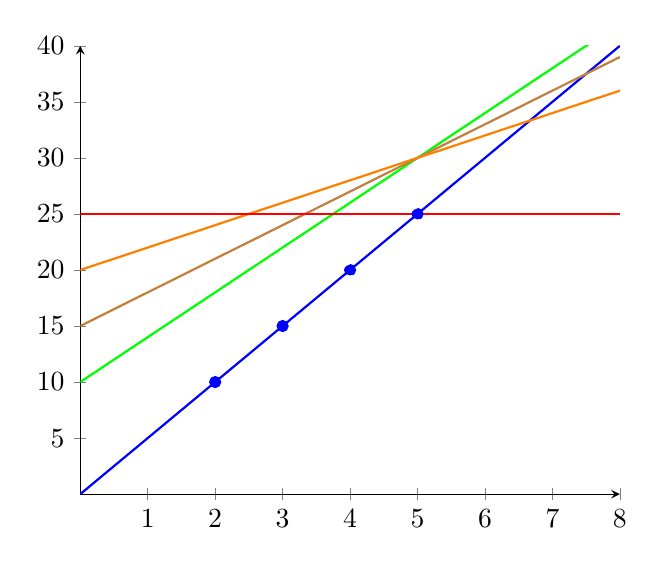
\begin{tikzpicture}
            \begin{axis}[
                axis lines = middle,
                label style = {below left},
                xmin=0, xmax=8, xtick distance={1},
                ymin=0, ymax=40, ytick distance={5}]
                \addplot+[mark=none,visible on=<2->][blue, solid, thick, domain=0:8] {5 * x + 0};
                \addplot+[mark options=blue,mark=*,only marks,samples at={2},visible on=<3>] {5 * x + 0};
                \addplot+[mark=none,visible on=<4->][green, solid, thick, domain=0:8] {4 * x + 10};
                \addplot+[mark options=blue,mark=*,only marks,samples at={3},visible on=<5>] {5 * x + 0};
                \addplot+[mark=none,visible on=<6->][brown, solid, thick, domain=0:8] {3 * x + 15};
                \addplot+[mark options=blue,mark=*,only marks,samples at={4},visible on=<7>] {5 * x + 0};
                \addplot+[mark=none,visible on=<8->][orange, solid, thick, domain=0:8] {2 * x + 20};
                \addplot+[mark options=blue,mark=*,only marks,samples at={5},visible on=<9>] {5 * x + 0};
                \addplot+[mark=none,visible on=<10->][red, solid, thick, domain=0:8] {0 * x + 25};
            \end{axis}
        \end{tikzpicture}
    \end{figure}
\end{frame}

\begin{frame}[plain,fragile]{Sample 2 - Illustrated}
    \begin{figure}
        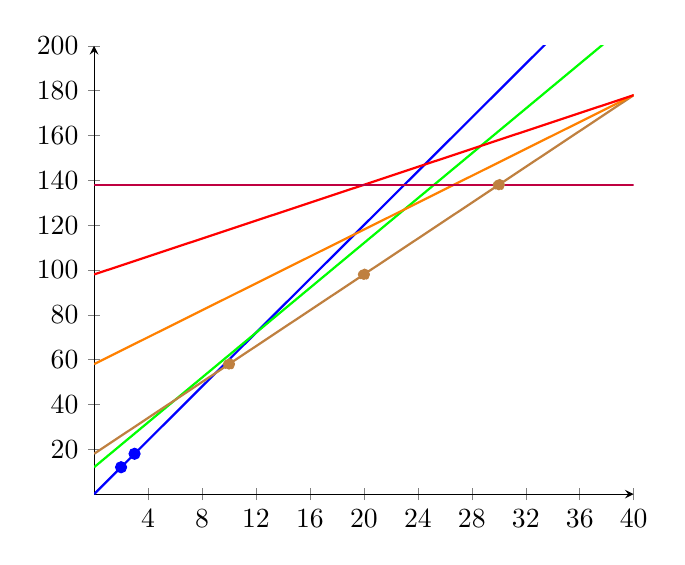
\begin{tikzpicture}
            \begin{axis}[
                axis lines = middle,
                label style = {below left},
                xmin=0, xmax=40, xtick distance={4},
                ymin=0, ymax=200, ytick distance={20}]
                \addplot+[mark=none,visible on=<2->][blue, solid, thick, domain=0:40] {6 * x + 0};
                \addplot+[mark options=blue,mark=*,only marks,samples at={2},visible on=<3>] {6 * x + 0};
                \addplot+[mark=none,visible on=<4->][green, solid, thick, domain=0:40] {5 * x + 12};
                \addplot+[mark options=blue,mark=*,only marks,samples at={3},visible on=<5>] {6 * x + 0};
                \addplot+[mark=none,visible on=<6->][brown, solid, thick, domain=0:40] {4 * x + 18};
                \addplot+[mark options=brown,mark=*,only marks,samples at={10},visible on=<7>] {4 * x + 18};
                \addplot+[mark=none,visible on=<8->][orange, solid, thick, domain=0:40] {3 * x + 58};
                \addplot+[mark options=brown,mark=*,only marks,samples at={20},visible on=<9>] {4 * x + 18};
                \addplot+[mark=none,visible on=<10->][red, solid, thick, domain=0:40] {2 * x + 98};
                \addplot+[mark options=brown,mark=*,only marks,samples at={30},visible on=<11>] {4 * x + 18};
                \addplot+[mark=none,visible on=<12->][purple, solid, thick, domain=0:40] {0 * x + 138};
            \end{axis}
        \end{tikzpicture}
    \end{figure}
\end{frame}

\begin{frame}[plain]{Remove useless lines}
    \begin{itemize}
        \item<1-> We can see some lines can be discarded, since they do not contribute to the convex hull.
        \item<2-> Suppose we are adding a line to our data structure.
        \item<3-> Let $a$ be the intersection point of the new line and the second to last line in the data structure.
        \item<4-> Let $b$ be the intersection point of the last line and the second to last line in the data structure.
        \item<5-> If the $x$-coordinate of $a$ is less than that of $b$, then the last line is redundant.
        \item<6-> We can therefore iteratively pop redundant lines from the back before adding a line.
    \end{itemize}
\end{frame}

\begin{frame}[plain,fragile]{Sample 2 - Remove useless lines}
    \begin{figure}
        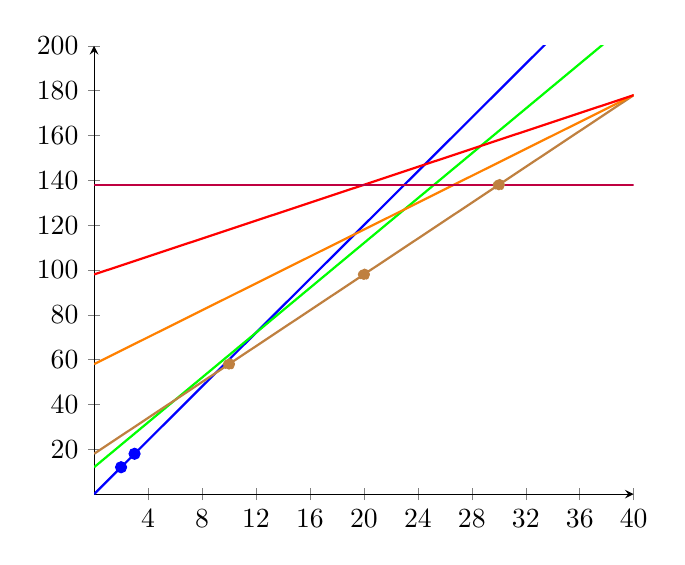
\begin{tikzpicture}
            \begin{axis}[
                axis lines = middle,
                label style = {below left},
                xmin=0, xmax=40, xtick distance={4},
                ymin=0, ymax=200, ytick distance={20}]
                \addplot+[mark=none,visible on=<2->][blue, solid, thick, domain=0:40] {6 * x + 0};
                \addplot+[mark options=blue,mark=*,only marks,samples at={2},visible on=<3>] {6 * x + 0};
                \addplot+[mark=none,visible on=<4-6>][green, solid, thick, domain=0:40] {5 * x + 12};
                \addplot+[mark options=blue,mark=*,only marks,samples at={3},visible on=<5>] {6 * x + 0};
                \addplot+[mark=none,visible on=<6->][brown, solid, thick, domain=0:40] {4 * x + 18};
                \addplot+[mark options=brown,mark=*,only marks,samples at={10},visible on=<8>] {4 * x + 18};
                \addplot+[mark=none,visible on=<9-11>][orange, solid, thick, domain=0:40] {3 * x + 58};
                \addplot+[mark options=brown,mark=*,only marks,samples at={20},visible on=<10>] {4 * x + 18};
                \addplot+[mark=none,visible on=<11-14>][red, solid, thick, domain=0:40] {2 * x + 98};
                \addplot+[mark options=brown,mark=*,only marks,samples at={30},visible on=<13>] {4 * x + 18};
                \addplot+[mark=none,visible on=<14-15>][purple, solid, thick, domain=0:40] {0 * x + 138};
            \end{axis}
        \end{tikzpicture}
    \end{figure}
\end{frame}

\begin{frame}[plain]{Querying and Complexity}
    \begin{itemize}
        \item<1-> How do we find the minimum $y$ value then?
        \item<2-> The intersection points are in ascending order.
        \item<3-> Use binary search to find the line in question.
        \item<4-> Construction takes $\mathcal{O}\left(n\right)$ time
        \item<5-> Each query takes $\mathcal{O}\left(\log n\right)$ time.
        \item<6-> We have improved the time complexity from $\mathcal{O}\left(n^{2}\right)$ to $\mathcal{O}\left(n \log n\right)$.
    \end{itemize}
\end{frame}

\begin{frame}[plain]{Modifications}
    \begin{itemize}
        \item<1-> Our current model only works if lines are inserted increasing/decreasing order by slope, but query points can be given in any order.
        \item<2-> Easy to change from minimization to maximization.
        \item<3-> If query points are also known to be in ascending order, you can use a sliding window idea to get $\mathcal{O}(n)$ time complexity.
        \item<4-> Alternatively, modify such that lines may come in any order while maintaining time complexity.
        \item<5-> Use a multiset instead of a vector/array to keep track of lines and quickly find insertion point. A bit more hassle but powerful.
        \item<6-> Need to consider removing neighbouring lines with higher and lower slopes.
    \end{itemize}
\end{frame}

\begin{frame}[plain,fragile]{Try on these problems!}
    \begin{itemize}
        \item \href{https://codeforces.com/contest/319/problem/C}{Kalila and Dimna in the Logging Industry}
        \item \href{https://open.kattis.com/problems/coveredwalkway}{Covered Walkway} (
        \item \href{https://dmoj.ca/problem/apio10p1}{Commando}
        %\item \href{https://open.kattis.com/problems/avoidingairports}{Avoiding Airports}
        %\item \href{https://open.kattis.com/problems/yatp}{YATP}
    \end{itemize}
\end{frame}

\section*{Divide and Conquer Optimization}



\end{document}

